\documentclass[12pt]{article}
 \usepackage[margin=1in]{geometry}
\usepackage{amsmath,amsthm,amssymb,amsfonts}
\usepackage{bm}
\usepackage{graphicx}

\newcommand{\N}{\mathbb{N}}
\newcommand{\Z}{\mathbb{Z}}

\newenvironment{solution}[2][Solution]{\begin{trivlist}
\item[\hskip \labelsep {\bfseries #1}\hskip \labelsep {\bfseries #2.}]}{\end{trivlist}}
%If you want to title your bold things something different just make another thing exactly like this but replace "solution" with the name of the thing you want, like theorem or lemma or whatever

\begin{document}


\title{Homework 3}
\author{Due Date: March 30, 2018}
\date{}

\maketitle

\begin{solution}{1}
1) The input points $(x_1, x_2, x_3)$ $(y_1, y_2, y_3)$ can be $(1,2,3)$ $(-1, +1, -1)$. \\
2) The decision boundary is represented by blue line as is shown in fig. 1.\\
3) Greater. Without the feature vectors, the margin is $3-1 = 2$ while it is $\sqrt{(1-3)^2 + (1-9)^2} = \sqrt{68}$ with feature vectors. 
\begin{center}
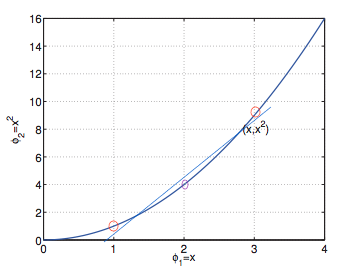
\includegraphics[angle = 0, width = .7\textwidth]{./images/fig1.png}
\end{center}

\end{solution}

\begin{solution}{2}
\begin{align*}
w = (0.5, 0.5)^T\\
b = -3.5
\end{align*}
The equation corresponding to the decision boundary is $0.5x_1 + 0.5x_2 - 3.5 = 0$. \\
The cordinates of the support vectors are (2,3) and (4,5) which are located in red circles as is shown in fig. 2. The decision boundary is the line $0.5x_1 + 0.5x_2 - 3.5 = 0$ marked in blue in the fig. 2. \\
\begin{center}
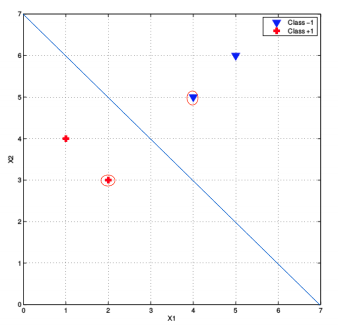
\includegraphics[angle = 0, width = .7\textwidth]{./images/fig2.png}
\end{center}
\end{solution}

\begin{solution}{3}
\begin{align*}
e^{- \gamma ||x - y ||_{2}^2} = e^{- \gamma ||x||_{2}^{2}}e^{- \gamma ||y||_{2}^{2}}e^{ 2\gamma x^{T}y}\\
= e^{- \gamma ||x||_{2}^{2}}e^{- \gamma ||y||_{2}^{2}} (1 + 2\gamma x^{T}y + \frac{(2\gamma x^{T}y)^2}{2!} + \frac{(2\gamma x^{T}y)^3}{3!} + ...)\\
= e^{- \gamma ||x||_{2}^{2}}(1, \sqrt{2\gamma} x_1, \sqrt{\frac{(2 \gamma)^2}{2!}}x_2^{2}, ...)^{T} e^{- \gamma ||y||_{2}^{2}}(1, \sqrt{2\gamma} y_1, \sqrt{\frac{(2 \gamma)^2}{2!}}y_2^{2}, ...)\\
= \phi(x)^{T}\phi(y)
\end{align*}
Therefore, the mapping function $\phi(x)$ is
\begin{align*}
\phi (x) = e^{- \gamma ||x||_{2}^{2}}(1, \sqrt{2\gamma} x_1, \sqrt{\frac{(2 \gamma)^2}{2!}}x_2^{2}, ...)^{T}
\end{align*}
\end{solution}
\end{document}